
\section{Introduction}
\label{sec:intro}
%\WF\, transiting planets are interesting because they are farther away
%and they have the possibility for measuring TTVs. Most everything else
%is possible with K2.

The \kep\ mission \citep{Borucki10} ushered in a revolution in our
understanding of exoplanetary systems in the Milky Way.
\kep\ observed a 100 deg$^2$ region of the sky in Cygnus and Lyra for
four years, detecting thousands of transiting planet candidates
\citep{Batalha13, Burke14, Mullally15, Rowe15}.  These planets include
populations largely undetectable by any other mission. For example,
with its high photometric precision, \kep\ has uncovered a population
of systems of tightly-packed inner planets (STIPs), with multiple 1-4
\rearth\ planets all transiting the same star with periods shorter than
$\sim 20$ days. These planets are largely too small to be detected by
other transit missions and too lightweight to be detected by RV
surveys.

In further contrast to radial velocity surveys \citep[e.g.][]{Udry07,
  Ford14}, which primarily targeted bright, nearby ($\lesssim 100$ pc)
FGK stars \citep{Valenti05, Ammons06}, \kep\, probes stars as faint as
$r = 16$. Hence, most \kep\, planet candidates are beyond 300 pc from
the Earth, with some as far as a kiloparsec away \citep{Lillo-Box14,
  Barclay15, Quinn15}.  The mission has found some surprising
differences between the local neighborhood and more distant regions of
the galaxy.  In particular, the number of hot Jupiter systems
discovered by \kep\ suggests an occurrence rate approximately 50\% of
that suggested by RV detections of hot Jupiters in the solar
neighborhood.  RV surveys estimate an occurrence rate for hot Jupiters
on the order of 1\% \citep{Cumming08, Mayor11}, while data from the
\kep\ mission suggest an occurrence rate of $0.4\% \pm 0.1\%$
\citep{Howard12}.  
While the difference between the two fields is known, the
explanation is unclear. Studies have invoked stellar metallicity
\citep{Howard12, Wright12, Dawson13}, stellar age \citep{Schlaufman13}, and
stellar multiplicity \citep{Wang14, Wang15a}. Regardless, this result
suggests that planet occurrence rate may be affected by the local
galactic environment. 

Aside from this result, so far, comparative studies of exoplanet
demographics as a function of galactic environment have been limited.
One of the first comparisons in planet occurrence across the galaxy
was afforded by microlensing surveys, which is biased toward low-mass
host stars at $\sim$kpc distances. 
\citet{Clanton14b} 
combined microlensing results
\citep[e.g.][]{Sumi10,Gould10,Cassan12} with those from RV and 
adaptive optics imaging surveys
\citep{Montet14} to show that the occurrence rate of giant
planets around M dwarfs is consistent as measured by the two
techniques. However, the microlensing signal from a planet is a much
less steep function of mass than the RV signal ($\propto \sqrt{m_p}$
and $\propto m_p$, respectively). At the
same time, the radius function around M dwarfs is strongly biased toward
smaller mass planets \citep{Swift13, Morton14}. Hence,
both \citet{Clanton14b} and \citet{Montet14} concluded that M dwarf planets
are explained by a steep mass function and most RV surveys miss the
$\sim$Saturn-mass, long period planets that likely make up the bulk of
the microlensing detections.

The \KT\ mission is providing a first opportunity to understand the
differences in planet populations across the galaxy for larger planets
and higher mass stars.  Due to the failure of two reaction wheels on
the \kep\ telescope, the instrument is no longer able to point at its
original field.  Instead, it relies on solar radiation pressure and
its remaining two reaction wheels to point at a series of fields in
the ecliptic plane for $\sim 70$ days at a time.  This new mission has
led to catalogs of transiting planet candidates
\citep{Foreman-Mackey15, Vanderburg16} as well as statistically
validated planets \citep{Montet15b} in fields across the ecliptic
plane.  By the end of the \KT\ mission, it will observe $\sim 20$
fields, largely covering the ecliptic plane, providing an opportunity
to probe variations in planet occurrence as a function of galactic
position and stellar age.

The upcoming \textit{TESS} mission \citep{Ricker14} will enable additional
detections of systems of small transiting planets, especially towards
the ecliptic poles where observations will be collected,
uninterrupted, for nearly a year.  However, \textit{TESS} is designed to
target stars brighter than $I = 12$, meaning most planetary detections
will be around stars within a few hundred parsec.  While ideal for
detecting the nearest planets, \textit{TESS} will provide little information
about their distribution in the galaxy.

\WF\ \citep{Spergel15} offers a unique opportunity to understand the distribution
of short-period transiting planets in our
galaxy.
During the mission,
six microlensing campaigns spread over five years will each last 72 days.
\WF\ will tile 2.8 square degrees of the sky
towards the galactic bulge with ten pointings.
Each pointing will be observed for 52 seconds every 15 minutes
While the photometric precision will not be as good for bright
stars as the \kep\ prime mission, its performance is signficantly
better for faint stars, of which \WF\, will observe millions
\ref{fig:noise}. \citet{BennettRhie02} showed that such a survey
should detect large numbers of transiting planets, especially giant
planets.
In a white paper in \citet{Spergel15}, Tanner \& Bennett calculate that \WF should see
50,000 transiting Jupiters.

\WF\ provides an opportunity to explain the discrepancy between the occurrence rate of hot Jupiters
in the \kep\ field and the solar neighborhood. 
\WF\ will observe stars at large distances along the galactic 
metallicity gradient \citep{Rolleston00, Pedicelli09}. 
Observations suggest a change in the metallicity of -0.05 dex/kpc as one moves
radially outward from the center of the galaxy.
\WF\ should be expected to observe stars at preferentially higher metallicities than
the solar neighborhood.
Indeed, simulations of the \WF\ field suggest the median G2V dwarf observable by \WF\ with W149 < 19.5 has
[Fe/H] = 0.26 \ref{ss:yield}.
The yield of hot Jupiters detected will provide key insights into the nature of the
formation and evolution of these massive planets.

The potential of \WF\, to detect large numbers of transiting planets
is under-appreciated because of the difficulty of confirming and
validating those planets. In general, because the host stars of
\WF-detected transiting planets will be so faint, it will not be
possible to conduct followup RV observations to confirm their
masses. This poses a major challenge for distinguishing transiting
Jupiter-radius planets from the multitude of false positives. However,
there are several techniques based on \WF\, data alone that can be
used to rule-out false positives. For example, \citet{McDonald14}
explore observations of Doppler beaming and secondary eclipses
as means to rule-out
transiting planet false positives for the proposed \textit{Euclid}
microlensing survey.

In this paper, we consider the capability of the upcoming \WF\ mission
to detect, confirm, and characterize transiting planets. In
particular, we focus on the possibility of measuring their transit timing variations \citep[TTVs,][]{Agol05, Holman05,LithwickWu12}. We
also discuss various techniques for ruling out false positives. In
Section \ref{sec:kepler}, we describe the mission photometry and compare it to \kep. 
In Section 8.3, we study
the sensitivity of \WF\ to detecting transit events and measuring
times of transit. 
In Section 8.4, we project the yield and demographics of transiting planets \WF\ will 
discover. In Section 8.5, we discuss potential strategies to
confirm the transiting planets discovered by \WF.  In Section 8.6 we discuss 
methods to statistically validate planets which can not be directly confirmed and
the potential for ground-based follow-up and strategies to maximize the
scientific potential of \WF\ for transiting planets. 
We conclude in Section 8.7.

\section{Comparison to \kep\ Photometry}
\label{sec:kepler}

To detect microlensing events, \WF\ requires a long time baseline to stare at fields
in the bulge, high photometric precision, and a wide field of view in order to observe
large numbers of stars.
Fundamentally, these are the same requirements as space-based transit surveys such as \kep.
We compare the expected performance of \WF\ with the actual
performance of \kep.
Such an analysis enables us to understand the detectability of transiting planets
potentially
observable by \WF\ 
as the requirements are similar and the statistics of planets discovered by the \kep\ 
mission are well-understood.


For unsaturated stars ($H > 15$), we calulate the photometric precision as a function of stellar magnitude, following
the standard CCD signal to noise equation. We use the values from the science definition team (SDT) report \citep{Spergel15}
for the photometric zeropoint of the
detector, as well as the bias, read noise, gain, dark current, and sky brightness. 
This report claims an error floor in the photometry of 1 mmag, which we add in quadrature to
the calculations from the SDT. This prescription is shown as the black line in Figure \ref{fig:noise}.


We compare this prescription to that of \citet{Gould15}, who
consider \WF\ as a tool for asteroseismology, especially
for saturated stars.
They perform their own analysis of the expected photometric precision and find that the precision in a single observation will scale such that
\begin{equation}
\sigma = 1.0 \times 10^{(2/15)m_H} \textrm{mmag},
\end{equation}
where $M_H$ is the apparent $H$-band magnitude. 
Taking W149 as a proxy for H, we also plot this relation on Figure \ref{fig:noise} (red line).


We show the results of this calculation and compare to \kep\ photometry in Figure \ref{fig:noise}.
To perform a direct comparison to \kep, we must make two corrections. 
First, \WF\ will observe at a faster cadence than \kep. 
To compare the observations in a uniform way, we follow the \kep\ convention of considering
the average noise of observations binned over six hours, the ``combined differential 
photometric precision'' or CDPP \citep{Christiansen12}.
Additionally, the \WF\ bandpass is significantly redder than the \kep\ bandpass. 
As transit searches focus on FGKM stars, with red colors, these stars appear brighter on the
\WF\ detector than they would on the \kep\ detector.
To provide a fair comparison, we compare the expected \WF\ precision to the H-band magnitude
of the stars in the \kep\ field.

Between 15th and 20th magnitude, the SDT estimates of the precision is very similar to
that of \citet{Gould15}.
In both cases, the expectation is that \WF\ will achieve a relative precision of 1 part per 
thousand (ppt) in a single observation of a 15th magnitude star in the 
W149 bandpass (0.93-2.00 $\mu m$). This is equivalent to 200 parts per million 
(ppm) when binned over six hours, comparable to the precision of \kep\ on a star
with $r \approx K_p =15$. However, since a typical G dwarf has an $R-H$ color of 1.1, 
the same Sunlike star observed with \kep\ and \WF\ would be observed at
a higher precision with \WF.

In this work, we focus on the detection of planets around stars with W149 $< 19.5$. The two
prescriptions for the photometric noise around such bright stars differ significantly only for stars
brighter than 14th magnitude. 
As these stars make up only a small fraction of the stars in the \WF\ field of view, the choice of
noise model we apply does not affect our results at an appreciable level. 
For ease of reproducability we apply the \citet{Gould15} model, noting the results change at only
the 1-3\% level (higher for stars of earlier spectral type) if we apply the \citet{Spergel15} model
instead.

\begin{figure}[htbp!]
\centerline{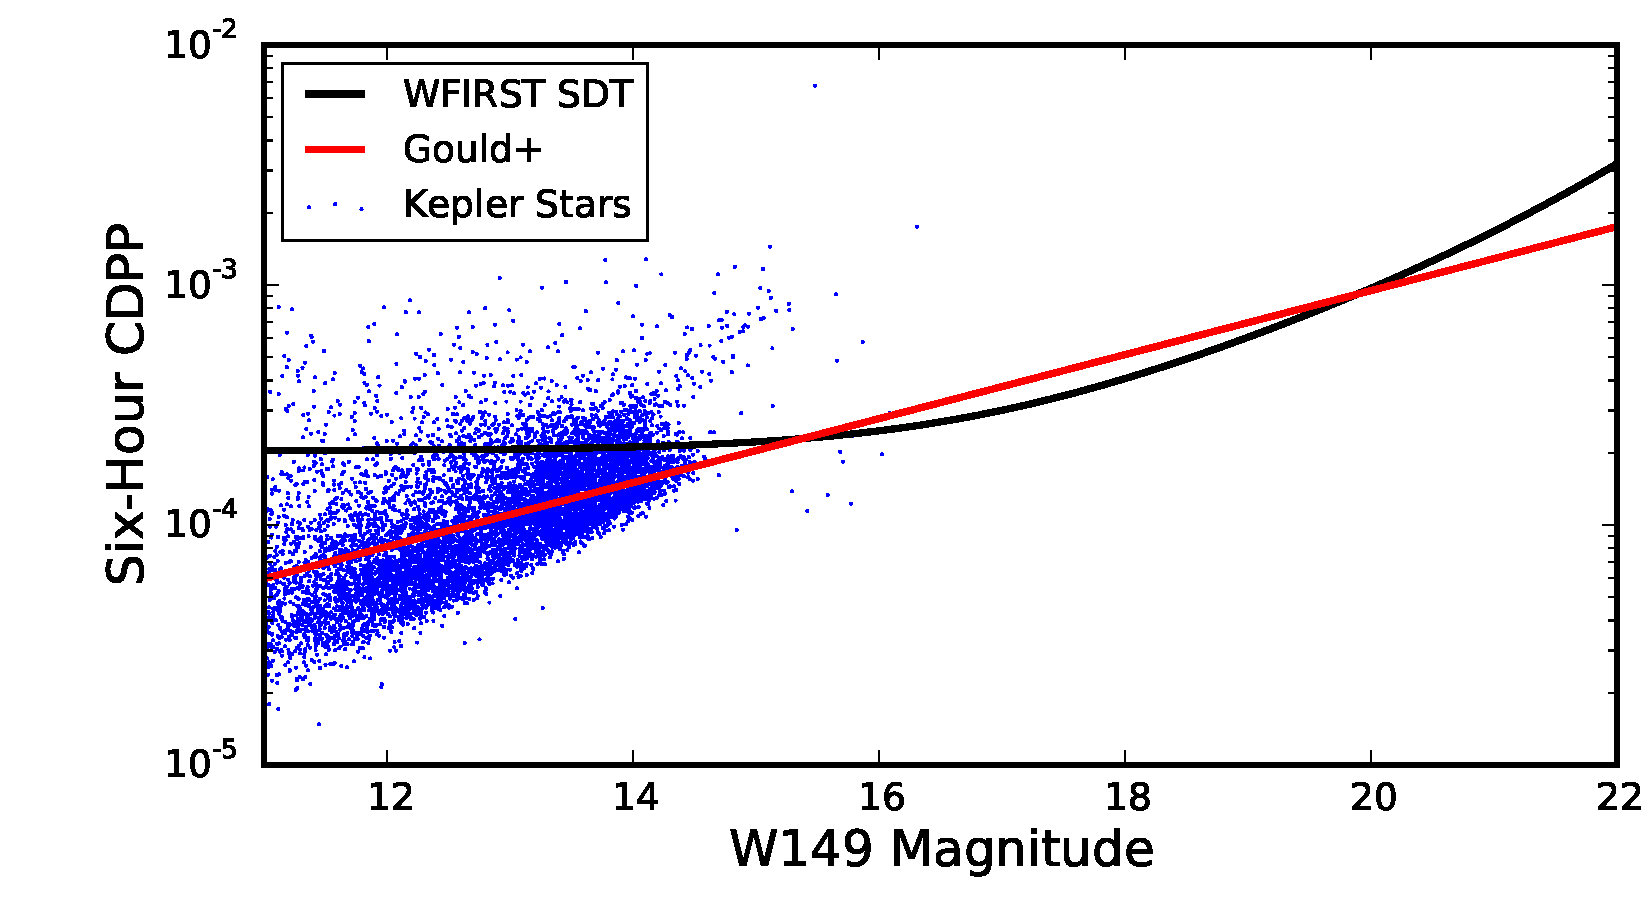
\includegraphics[width=0.75\textwidth]{chapter8/f1.pdf}}
\caption[Expected noise properties of \WF\ observing in the W149 bandpass as a function of
stellar magnitude]{Expected noise properties of \WF\ observing in the W149 bandpass as a function of
stellar magnitude. The black curve represents the estimates of the noise properties from the
\WF\ SDT report. The red curve represents the estimates of the noise properties from 
\citet{Gould15}, who focus on saturated stars to detect asteroseismic modes using \WF\ data.
In blue are actual observations of stars from \kep\ for comparison. In all cases, we report
the six-hour CDPP, or the noise averaged over six hours of observations.}
\label{fig:noise}
\end{figure}



\section{Detection of Transit Events}
\label{sec:transits}

To study the detectability of transiting planets with \WF, we
simulate transiting planet light curves with properties based on the
anticipated performance of \WF\, as described by \citet{Gould15}. We
assume a 52-second integration every 5 minutes and 6 evenly-spaced,
72-day campaigns over five years. We assume that all data will be
taken in the W149 band ($\textrm{0.927--2.000}\mu$m) with the exception of one data point
every 12 hours in the Z087 filter
($\textrm{0.760--0.977}\mu$m), i.e.\ one Z087 data point for every 47 obtained
in W149.

In this work, we assume the photometric noise is white, so that there are no correlations
between observations. 
Correlated noise can be the result of spacecraft systematics or stellar p-modes 
\citep{Gilliland10, Campante11}. 
The timescale for p-modes is inversely proportional with stellar density:
for G dwarfs, the granulation timescale is approximately five minutes; for M dwarfs, 
30 seconds. 
Like \kep\ data, for most stars observations will be 
spaced widely enough to capture a random phase of p-mode oscillations during each observation.
As \WF\ has significantly larger levels of photon noise, the correlated
stellar signals will be small by comparison, causing the while instrumental noise to dominate
over any red astrophysical effects.




\subsection{Hot Jupiters}
\label{sec:HJ}

The \WF\ microlensing mission intends to target more than one million stars
with $H < 14$ and 12 million stars with $H < 19$. To better understand the 
sensitivity of \WF\ to giant transiting planets, we simulate transits of a hot Jupiter
transiting a Sunlike star. 

We simulate individual transits of a hot Jupiter by injecting both realistic noise
and a planetary signal into simulated \WF\ data. We first create a star with
W149 $= 15.0$ to project a best-case scenario, where the noise expected to be at
the milimagnitude noise floor.
We then inject a Jupiter-sized planet on a 3.0 day orbit around this star,
which transits with impact parameter $b = 0.5$. 
The transit duration is approximately two hours.
Every fifteen minutes, starting at a random phase, we collect an observation
of the flux from this system: every twelve hours one observation is taken in 
Z087, while all other observations are in W149. 
We model the transit light curve with the transit model of \citet{Mandel02}. 
We calculate limb darkening coefficients in each bandpass using the online tool
developed and described in \citet{Eastman13}, which interpolates the 
\citet{Claret11} quadratic limb darkening tables. 

Unlike the \kep\ mission, each data point will consist of a single 
52-second observation, rather than a series of binned observations over 30 minutes.
Each observation will then sample one specific point on the transit light curve
as opposed to an integrated measure of the observed flux, meaning morphological
light curve distortions due to finite integration time will be virtually nonexistant in
\WF\ data \citep{Kipping10}.

The resultant ``observed'' transits are shown in Figure \ref{fig:HJtrans}.
These transits can be seen by eye, even in the case of single transit events.
Over the course of the mission, more than 150 transits of such a Hot Jupiter would be observed, leading
to approximately 1200 observations during the transit in the W149 bandpass.
Moreover, approximately two dozen observations during the transit will be collected
in the W089 bandpass, which might be useful for confirmation of the planetary 
nature of this signal (Section \ref{sec:confirm}).


\begin{figure}[htbp!]
\centerline{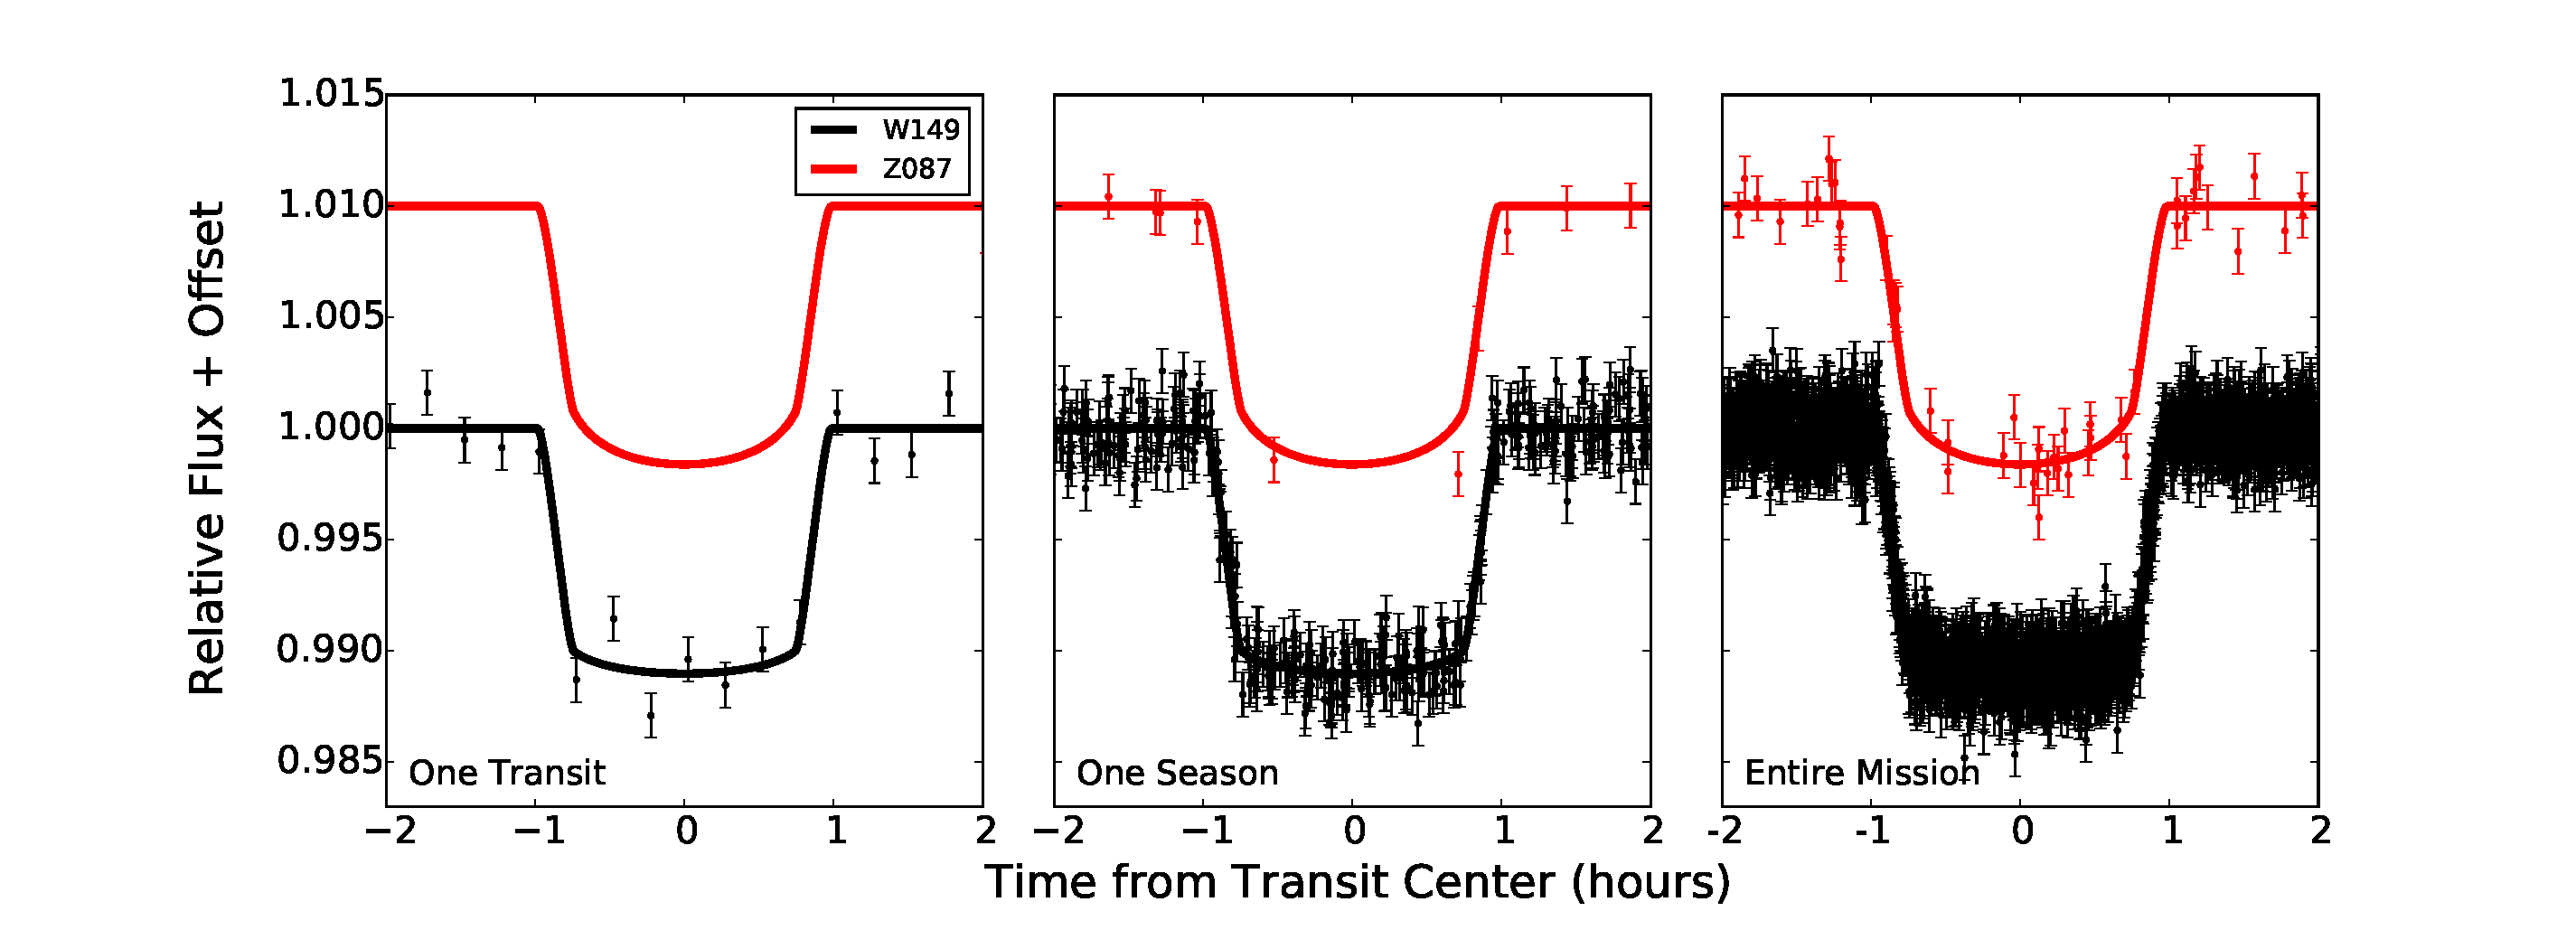
\includegraphics[width=0.9\textwidth]{chapter8/f2.pdf}}
\caption[Simulated transit photometry for a hot Jupiter in a three-day orbit
around a Sun-like star as observed with \WF.]{Simulated transit photometry for a hot Jupiter in a three-day orbit
around a Sun-like star with W149 $= 15$. In black is photometry from the
W149 bandpass; in red, the Z087 bandpass. The left panel corresponds to a single
transit. The middle panel corresponds to transits folded together over a 72-day
observing season, while the right panel corresponds to six such seasons over the
course of the mission.}
\label{fig:HJtrans}
\end{figure}

We then attempt to recover the transit signal in the data. By fitting transit
models and evaluating their likelihood, we measure a transit depth of
$0.998 \pm 0.002$ $R_J$, assuming perfect knowledge of the stellar host. 
This $\sim 500 \sigma$ detection of a transit implies
transiting hot Jupiters will be easily detected around $H \sim W149 = 15$ stars.

We can increase the level of the noise to determine the limiting magnitude
for which \WF\ will be effective at detecting hot Jupiters.
In the \kep\ mission, the threshold for a candidate planet transit was a $7.1\sigma$
detection of the transit, a standard we will apply here.
By inflating the size of our photometric uncertainties and repeating this exercise
we find that, assuming white noise, even when the single-point photometric precision
is 8\%, we are able to detect hot Jupiters in three-day orbits at $7.1 \sigma$ over
the course of the \WF\ mission.
The photometric limit is expected to be better than this value even
for stars with W149 $= 22.0$.
Typical extinction values in the $I$-band are 1-2 magnitudes \citep{Nataf13} and towards the 
galactic center $A_H/A_I = 3.2$, so we might expect less than one magnitude of
extinction in the W149 bandpass \citep{Nishiyama09, Nataf16}.
Even accounting for extinction, this limiting magnitude corresponds to Sunlike
stars well beyond $> 10$ kpc from the Earth, easily allowing us to detect hot Jupiter
systems around tens of millions of stars in total, at all Galactocentric radii.

For the brightest stars, measuring a transit signal to a precision of 
$0.2\%$ implies photometric precision of approximately 20 parts per million
when binned over two-hour intervals and phase-folded on a two-day period.
This is significantly below the precision needed to detect relativistic Doppler
beaming in the light curve \citep{Loeb03, Faigler11}, but could be used to detect
false positive events such as transiting brown dwarfs and low-mass stars masquerading
as hot Jupiters (see Section \ref{sec:PC}).


\subsection{Sensitivity to Small Planets}
\label{sec:small}

Given the high signal to noise expected for hot Jupiters transiting the brightest stars
observed with \WF, we might expect the telescope to be sensitive to planets transiting
stars significantly smaller than Jupiter as well.
We can determine how small a planet would be detectable by \WF\ as a function of planet
orbital period and radius. 
We will repeat this exercise for stars at W149 $= 15$ and $\textrm{W149} = 19.5$; there are 
expected to be 1 million and 12 million stars brighter than these limiting magnitudes,
respectively.

To calculate our sensitivity to planets in general, we first create a planet with a radius and an orbital
period drawn from log-flat distributions over the ranges $[1, 16]R_{\oplus}$ and $[1,72]$ days, respectively. We then assign an impact parameter for each
transiting planet drawn from
a uniform distribution over the range $[0, 1]$. 
We assume a circular orbit for the planet and calculate the relative position of the 
planet and star, applying the transit model of \citet{Mandel02}.
We draw an observation every fifteen minutes.
We assume white noise with the photometric
precision given by the \citet{Gould15} curve of Figure \ref{fig:noise}, removing one observation every twelve hours
when \WF\ is collecting $z$-band data instead.
After all transits have been simulated, we phase-fold on the known period and measure
the significance of the observed transit depth. 
If it is larger than $7.1\sigma$, we declare this transit detected; otherwise, we declare
it missed.
We also require at least two transits during at least one season to be detected.
By repeating this procedure many times with many different planet sizes and periods,
we can map the sensitivity of \WF\ to small planets. The results are shown in Figure
\ref{fig:Sensitivity}.

\begin{figure}[htbp!]
\centerline{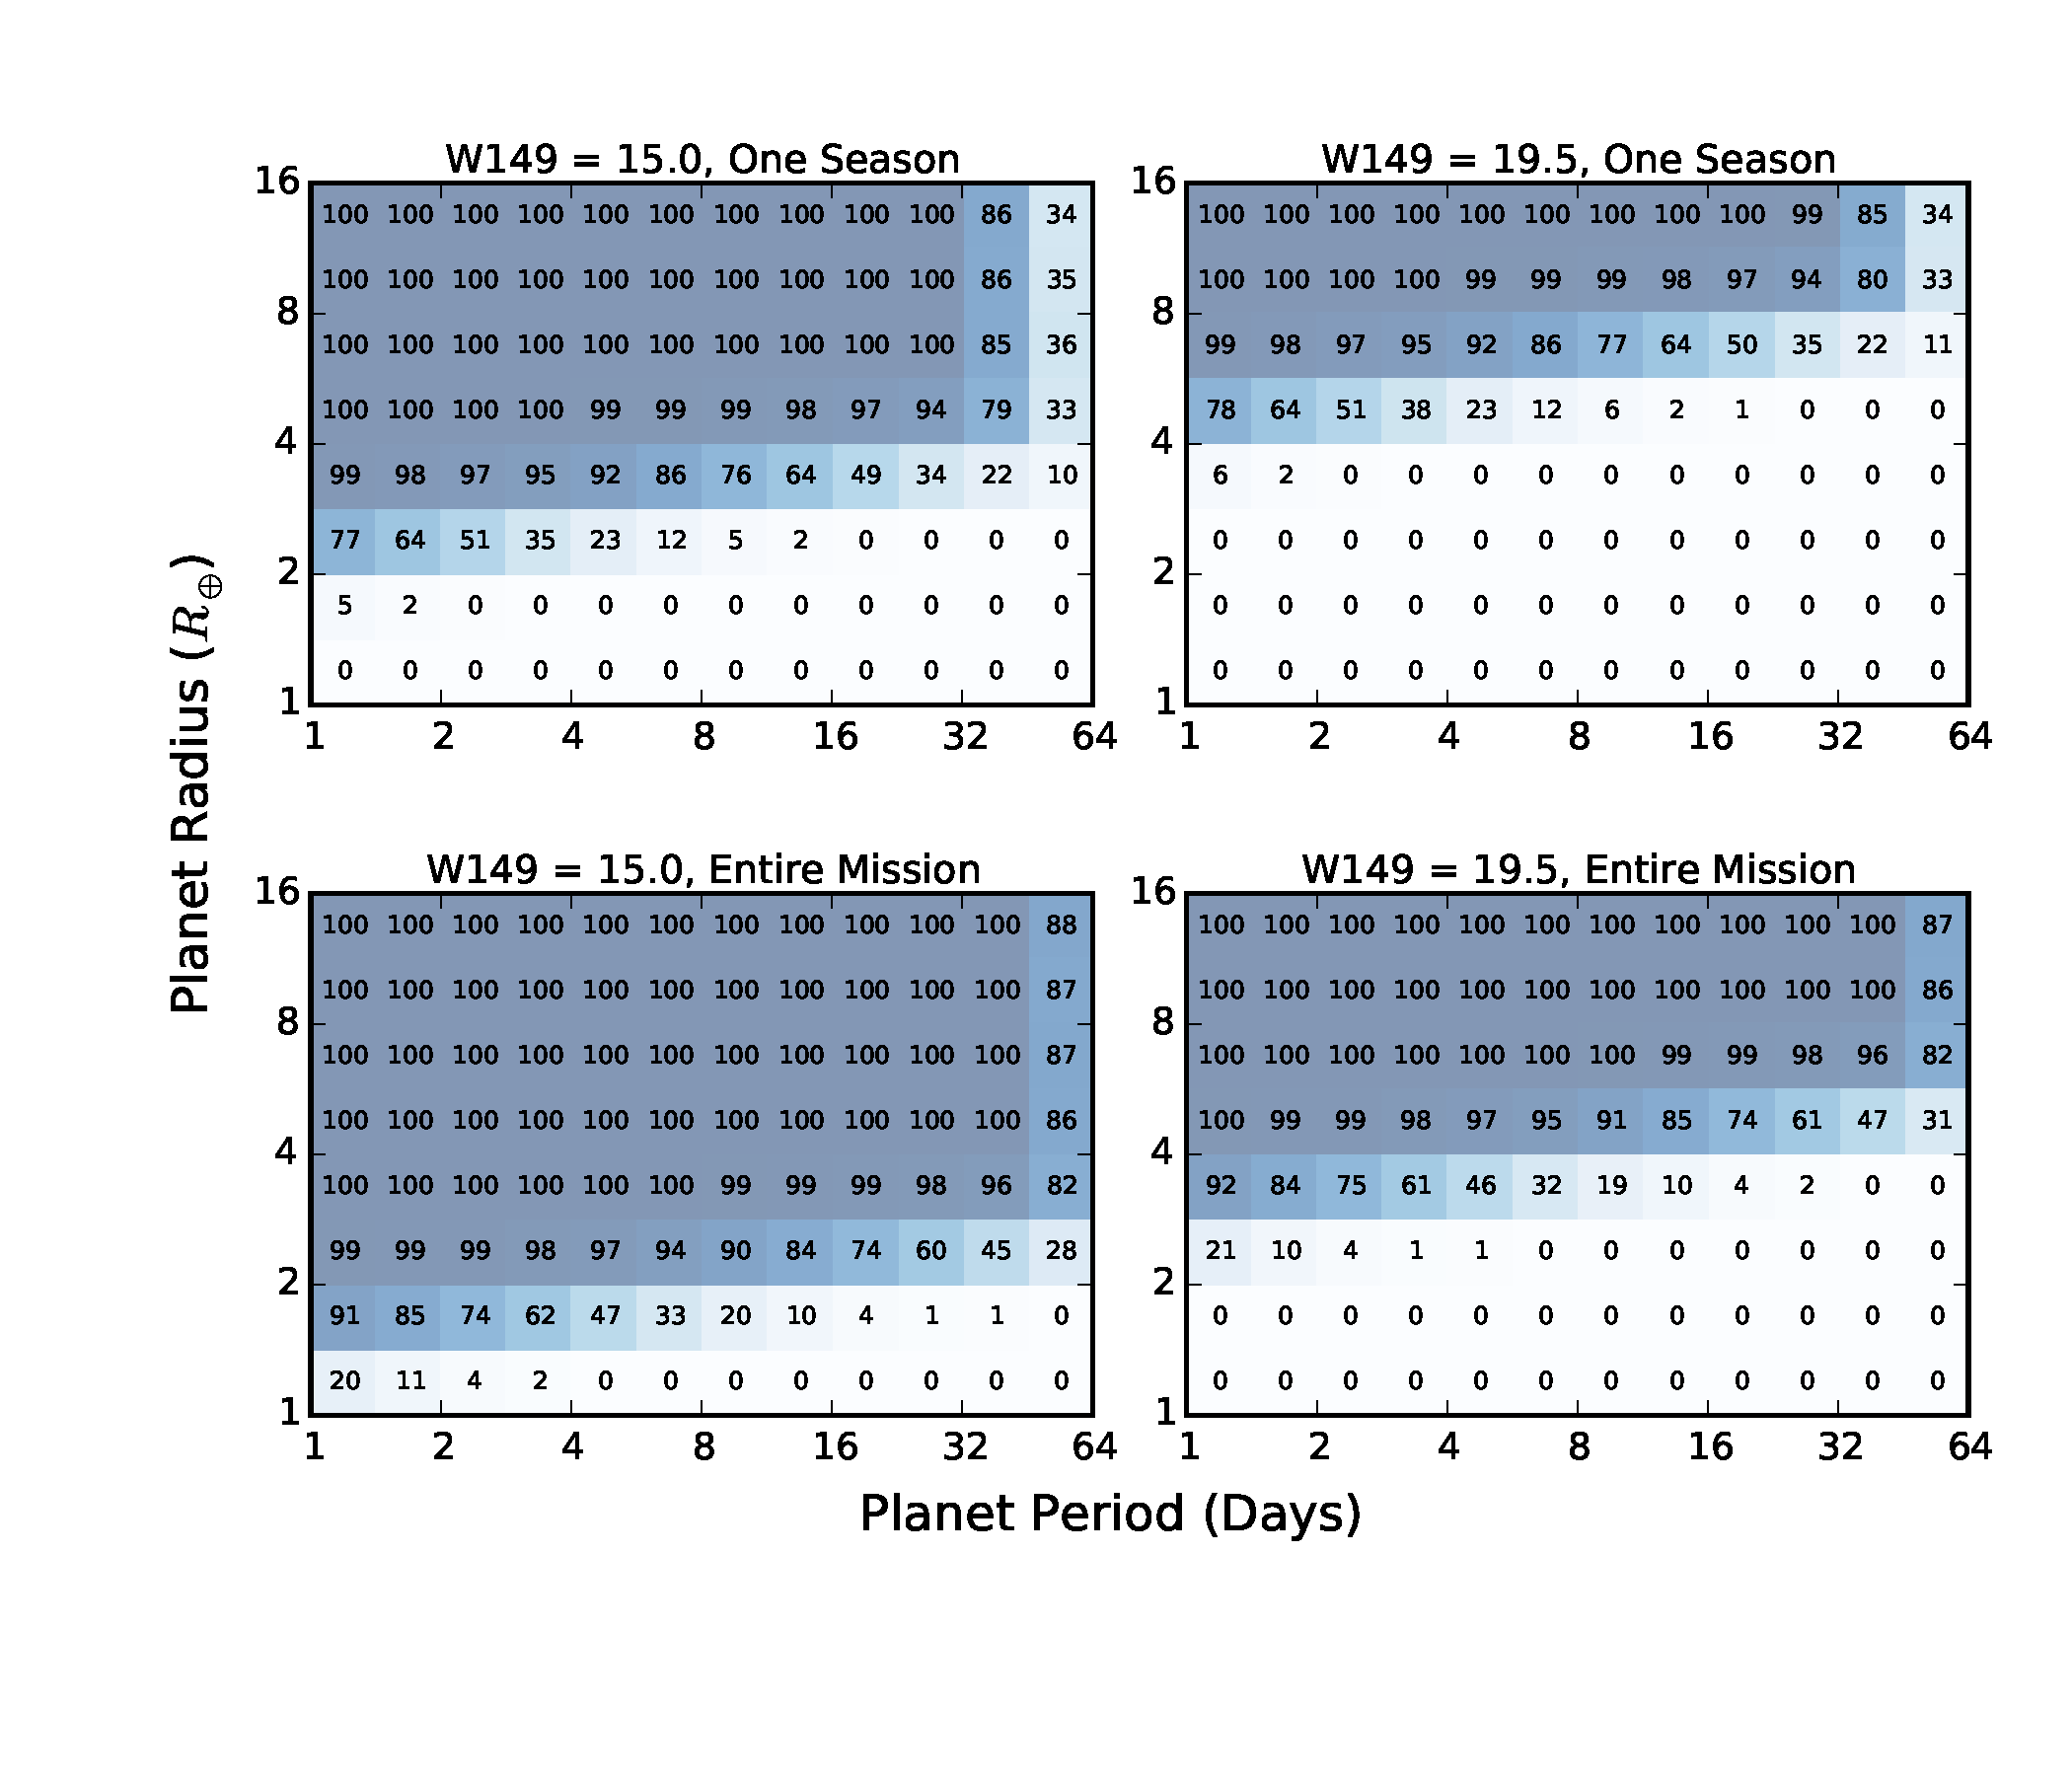
\includegraphics[width=0.98\textwidth]{chapter8/f4.pdf}}
\caption[Fraction of planets of given sizes and orbital periods expected to be detected by \WF.]{Detectability of planets transiting a Sunlike star in simulated \WF\ data by analyzing (top) one season of data and (bottom) data from the entire mission.
Around very bright stars (W149 = 15.0) nearly all Neptune-sized planets and larger with
orbital periods shorter than the seasonal baseline will
be detected in a single season of data.
To qualify as a detection, we require at least two transits in a single observing season,
but not necessarily in all seasons.
}
\label{fig:Sensitivity}
\end{figure}

We find that, for the brightest stars observed by \WF, Neptune-sized planets with
orbital periods shorter than one month will be easily detected in a single season of data. 
The mission will also recover many mini-Neptunes with periods shorter than 20 days, and
is likely to recover a small number of planets smaller than 2 \rearth\ with 
periods shorter than two days. 
Over the entire mission, \WF\ will be sensitive to a few Earth-sized planets 
with orbital periods shorter than two days orbiting the brightest stars.
Of the 12 million stars with $\textrm{W149} < 19.5$, the prospects for detecting super-Earths
or mini-Neptunes are much lower, but the mission will detect the majority of  
Neptune-sized planets with periods less than a month and all transiting Jupiter-sized
planets in that period range as well.

There is a strong decay in the sensitivity of \WF\ to transiting planets as a function
of planet radius compared to planet period. This is not surprising, and the same effect
is seen in \kep\ data \citep{Burke14, Mullally15, Rowe15}. 
The transit duration is proportional to $P^{1/3}$ and the observed depth
depends on the projected surface area of the planet, so
the phase-folded transit signal depends on $R_p^2 P^{-2/3}$ \citep{Seager03}. Therefore a change in the orbital period should have a weaker effect than a change in the size of the planet, as we
observe here \citep[see also][]{Carter08}.

\subsection{Single Transit Events}

\WF\ will, in addition to detecting thousands of planets with short orbital periods, be
sensitive to singly transiting events of giant planets in more distant periods.
The best measurements of the occurrence rates of these planets is understood from 
combining observations of long-term RV accelerations with direct imaging surveys 
\citep[Gonzales et al. in prep]{Montet14}. 
There are only a few dozen such planets detected in the \kep\ data, detected largely
through visual inspection \citep{Wang15b, Uehara16}. 
For a given planet in a long orbital period, the probability of transit is directly
proportional to the observing baseline.
The \WF\ observing baseline is a factor of four shorter than that of \kep, but as the
total number of stars observed by \WF\ is nearly two orders of magnitude larger than 
\kep, we expect visual inspection of \WF\ data to uncover on the order of one thousand
additional giant planets. 
As even single transit events can provide unique information about transiting planets
\citep{Yee08, Osborn16}, these data will 
improve our understanding of planets at wide separations.


\subsection{Deriving Transit Times from \WF\ data}
\label{sec:ttvs}



The sensitivity to short-period planets smaller than Neptune in a single season of 
\WF\ data implies that we may be able to detect variations in the time of transit
across the mission.
These transit timing variations (TTVs) have been used previously to confirm the 
planetary nature of transiting signals \citep{Holman10, Fabrycky12, Ford12TTV, Xie13}, 
to detect the presence of non-transiting
planets \citep{Ballard11, Nesvorny12, Nesvorny13}, and to infer masses and
eccentricities of planetary systems 
\citep{Hadden14, Jontof-Hutter15, Jontof-Hutter16}.
While TTVs have been observed in \KT\ data \citep{Barros15}, the short time baseline makes
these detections the exception rather than the rule.
Given that \WF\ will observe the same fields over five years, we might expect to detect 
deviations from a linear transit ephemeris if our sensitivity to transit times is small enough.

To this end, we simulate transit events in order to estimate the precision to which we will
be able to measure transit times. We model our benchmark system after Kepler-9b and Kepler-9c, the first planets confirmed via TTVs \citep{Holman10}.
We use orbital periods for the two planets of 19.2 and 38.9 days. 
Given that less massive planets more often exhibit TTVs than more massive planets 
\citep{Mazeh13}, we simulate planets near the bottom of our detectability
contours in order to understand the limits for detecting TTVs with \WF. Hence, we assume the two planets are mini-Neptunes with masses of $10$ \mearth\ and radii of $3$ \rearth. These are significantly smaller than the real Kepler-9 planets leading to smaller TTVs and larger uncertainty in the measured time of transit center.
We simulate transits of these planets orbiting a Sunlike star with W149 = 15.0, so that
the photometric precision on each data point is 1 part per thousand, assigning 
impact parameters at random. 

We focus on TTVs of the inner planet, because more transits will be observed over the course of the \WF\ mission.
We fit a transit model to the simulated data for the inner planet, fixing the limb darkening to that
expected for a Sunlike star in the H-band but allowing all other parameters to vary. The measured transit times are shown in Figure \ref{fig:ttv}.
Simulating many transits, we find a median uncertainty in the measured transit time
for each individual transit
of 28 minutes. 
We then phase-fold all observed transits inside an observing season, finding a median
uncertainty on the average time of the folded transit of 15 minutes (Figure \ref{fig:ttv}). 
Given the large number of observed TTV signals in \kep\ significantly larger than this
timing precision, we expect \WF\ to be able to efficiently measure TTVs.




\begin{figure}[htbp!]
\centerline{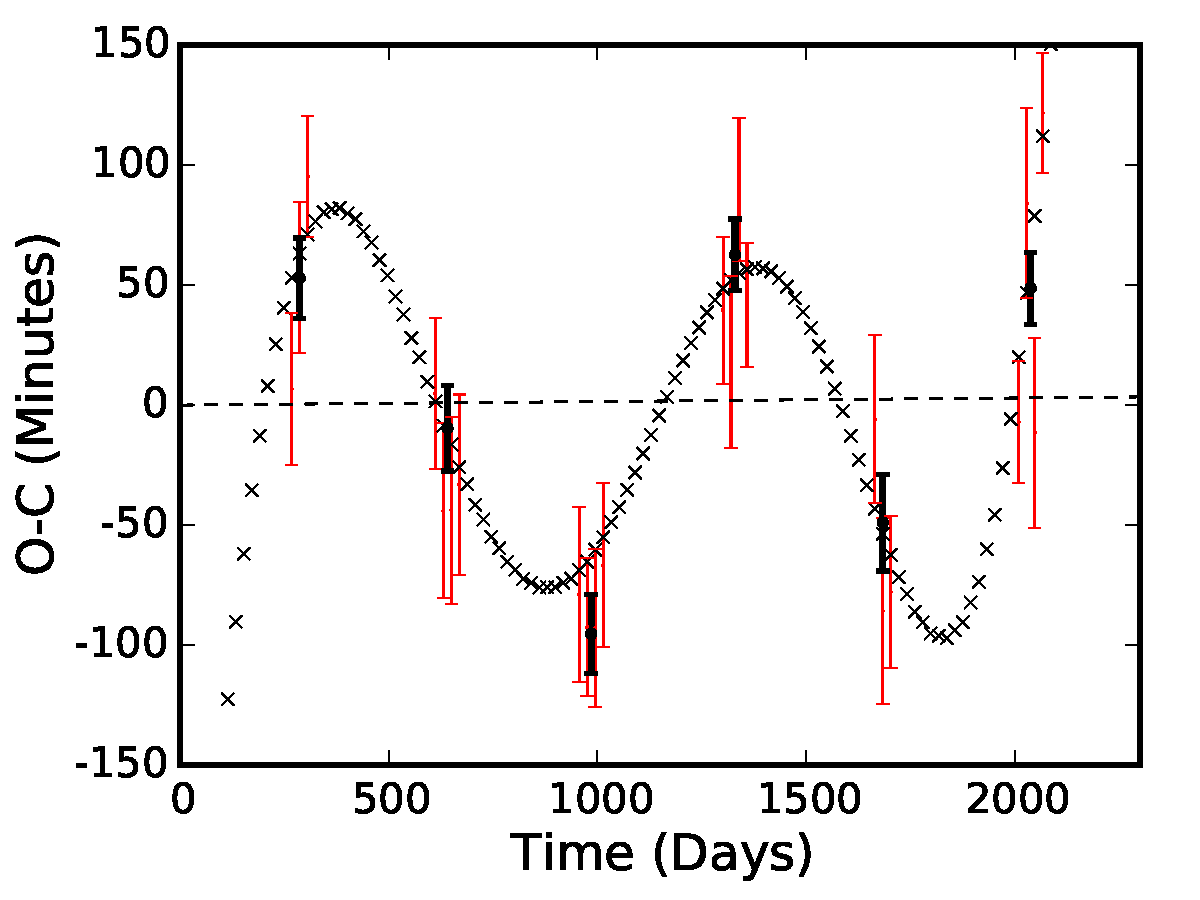
\includegraphics[width=0.75\textwidth]{chapter8/f3a.pdf}}
\caption[Simulated TTV signal from a two-planet system as observed by \WF.]{Simulated TTV signal from a two-planet system as observed by \WF\ (see Section \ref{sec:ttvs}). 
Gray X labels correspond to the actual deviation form a linear ephemeris for each 
individual transit. For those observed during a simulated \WF\ season, typical
uncertainties are added to the observed time of transit with data shown in red. The black
points correspond to binned observations over an entire season. This hypothetical system
would be confirmed by TTV observations in \WF\ data.}
\label{fig:ttv}
\end{figure}



Accurate determinations of transit times is more difficult in the presence of 
starspots, which induce a correlated signal in the light curve.
As a planet transits the stellar disk, if it passes across a 
relatively dark spot this will cause a distortion in the shape of the light curve.
Moreover, spots at other stellar latitudes can cause the out-of-transit flux baseline
to vary, complicating the measurement of the time of transit.
\WF\ will observe in the near-IR, where the effects of starspots are significantly 
minimized due to their lower contrast, reducing the possibility of significant 
starspot-induced timing errors.

\section{Galactic Exoplanet Demographics}
\label{ss:yield}


We can simulate realistic populations of both stars in the bulge and their exoplanets 
to estimate how many transiting planets \WF\ will be able to detect over the course of its mission.
To simulate a realistic estimate of the stellar population in the bulge, we develop a 
galactic population generated from the online Besan\c{c}on models of the galaxy \citep{Robin03}.
To convert the returned apparent magnitudes to near-infrared simulated photometry, we
apply the transformations of \citet{Bilir08}. 
We then apply a correction for interstellar extinction assuming the \citet{Cardelli89}
extinction law with $R_v = 2.5$, following \citet{Nataf13}.
From the derived JHK magnitudes, we approximate the W149 magnitude for each star
by assuming W149 = (J+H+K)/3.

We then apply a series of corrections to turn the Beasan\c{c}on models into a realistic
simulation of the stars observed by \WF. The Beasan\c{c}on model outputs the properties and numbers of stars along a given sightline within a certain solid angle.
Because each simulated field is not a perfect match to the \WF\ field, we weight each simulated star by the fraction of the simulated field that falls in the \WF\ field.
We then apply a correction for the mass function in the bulge. 
The model assumes stars in the bulge follow the Salpeter IMF \citep{Salpeter55}.
We downweight stars of mass $M< 0.5$ \msun\ by a factor of $0.5/M$, which approximates
the IMF of \citet{Kroupa01}.
We then apply a uniform correction to all stars to match the overall number of 
bulge main sequence stars near the \WF\ fields as measured by \citet{Calamida15}.

We then inject planets around the main-sequence
dwarf stars brighter than W149 = 19.5 in our simulation. Since the 
\WF\ sensitivity in the radius-period plane (Figure \ref{fig:Sensitivity}) is limited to a region of parameter space 
well-sampled by the \kep\ mission in the original \kep\ field.
We assign planets around solar-type FGK stars following the planet occurrence estimates 
of \citet{Howard12}.
We assign planet radii and orbital periods following the ``Cutoff Power-Law Model'' of Table 5 of
that paper, and bulk occurrence rates for each spectral type following the authors' Table 4.
For M dwarfs, we follow the relations of \citet{Morton14}, specifically their ``logflat+exponential''
model of the period distribution from their Figure 7 and the radius distribution from their Figure 6.
This leads to considerably smaller numbers of giant planets injected around M dwarfs than more massive
stars, in line with observations from \kep.

We simulate the transits of these planets following the same prescriptions as in Section \ref{sec:transits}.
We assume the noise properties of \citet{Gould15} and we estimate limb darkening parameters by interpolating our stellar parameters onto the
quadratic limb darkening grids of \citep{Claret11}, taking $H-$band as a proxy for W149. We limit the range of orbital periods to $P<72$ days.
We declare a planet detected if we 
recover its transit signal at $7.1\sigma$ and observe at least two transits in any one season.

The results are shown in Figure \ref{fig:yield1}. We expect \WF\ to detect approximately 13,000
transiting planets orbiting bright dwarf stars, the majority being giant planets orbiting F and G stars.
The mission will also detect more than 100 planets smaller than Neptune, the majority of which will
be orbiting M dwarfs. We note that our prescription for the photometric precision does not significantly affect the bulk numbers of planets detected.

The number of transiting planets from this simulation assumes that the occurrence rate is the same in the \WF\ field as in \kep.
However, radial velocity surveys have unveiled a correlation between giant planet occurrence and stellar 
metallicity \citep{Fischer05, Johnson10a}, while the presence of small transiting planets appear 
to not be affected by the host star's metallicity \citep{Buchhave15}. Given that the median metallicity of dwarfs in the \WF\ field is [Fe/H] = 0.25, and most of the planets detected by \WF\ will be giants, this correlation could significantly
influence the number of giant planets detected. 

We account for this metallicity effect by injecting planets according to the radius and period distribution of the
\kep\ field, but increasing the likelihood of a star hosting a planet according to the star's 
metallicity in our sample.
Following \citet{Johnson10a}, who find planet occurrence scales as $10^{1.2\textrm{[Fe/H]}}$, we 
modify the likelihood of all planets with radii larger than 5 \rearth\ by this factor.
For the median star ([Fe/H] = 0.25), this factor increases giant planet occurrence by a factor of two.
We then repeat our simulations with our modified planet occurrence, with the results shown in Figure \ref{fig:yield2}. 
In this case, we detect more than 30,000 transiting planets over the six seasons of the \WF\ mission.
As expected, the number of small planets is unchanged, with the gains made entirely in the
population of planets larger than Neptune. 
\WF, by completing this survey, will provide the best assessment of the effects of high 
metallicity on the population of giant planets, providing clues to the formation and evolution
of these systems.

Finally, we note that our analysis is limited to dwarf stars towards the bulge brighter
than W149 = 19.5. While planets have been detected
around evolved stars \citep{Lillo-Box14, Barclay15, Quinn15}, their occurrence rates
are too poorly understood to enable a reliable estimate of their yield in \WF. 
However, given the photometric precision (Section \ref{sec:kepler}) and scaling from Section \ref{sec:transits}, giant planets will be detectable around evolved stars (i.e. given that $3R_{\oplus}$ planets are detectable around a $1 R_{\odot}$ star, a $12R_{\oplus}$ planet should be detectable around a $4 R_{\odot}$ star.).
As \WF\ will observe large numbers of evolved stars towards the bulge, it will provide
the best measurement to date of the occurrence rate of giant planets in short orbits
around evolved stars.




\begin{figure}[htbp!]
\centerline{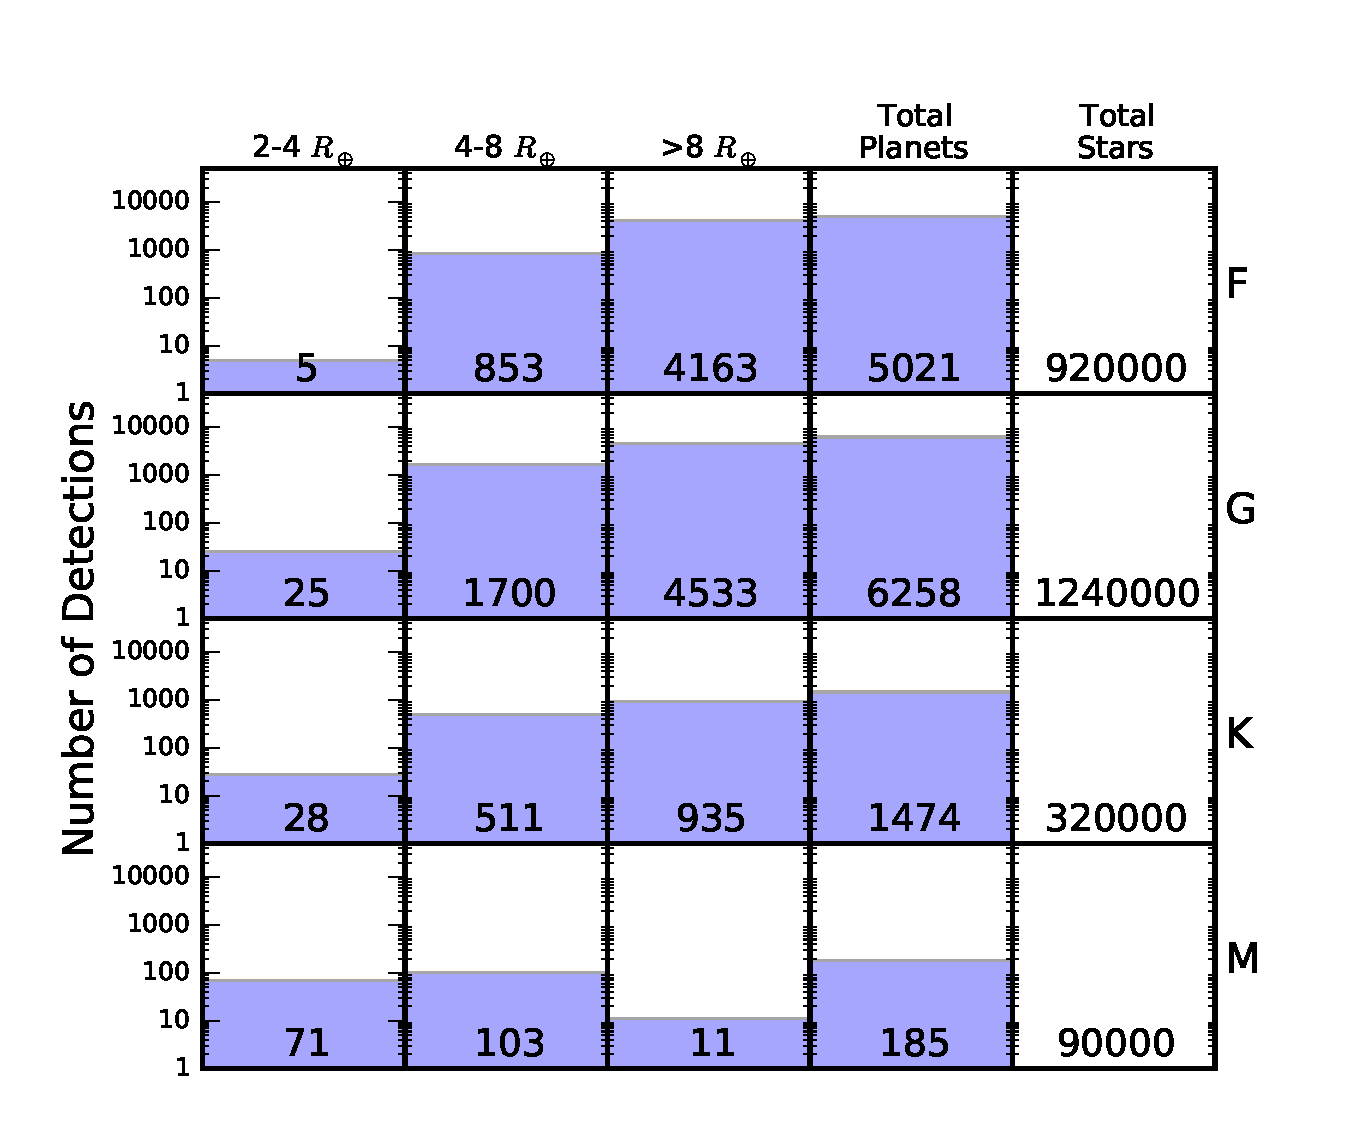
\includegraphics[width=0.75\textwidth]{chapter8/f5b_n.pdf}}
\caption[Expected transiting planet yield from \WF\ assuming planet occurrence is the same as that in
the \kep\ field]{Expected yield of transiting planets orbiting dwarf stars
  brighter than W149 = 19.5 in the \WF\ data as a function of
  planet size and stellar type, assuming the planet occurrence is the same as that in the \kep\ 
  field. \WF\ will detect thousands of Jupiter sized planets, but also more than 100 planets
  smaller than Neptune, mainly around M dwarfs. }
\label{fig:yield1}
\end{figure}


\begin{figure}[htbp!]
\centerline{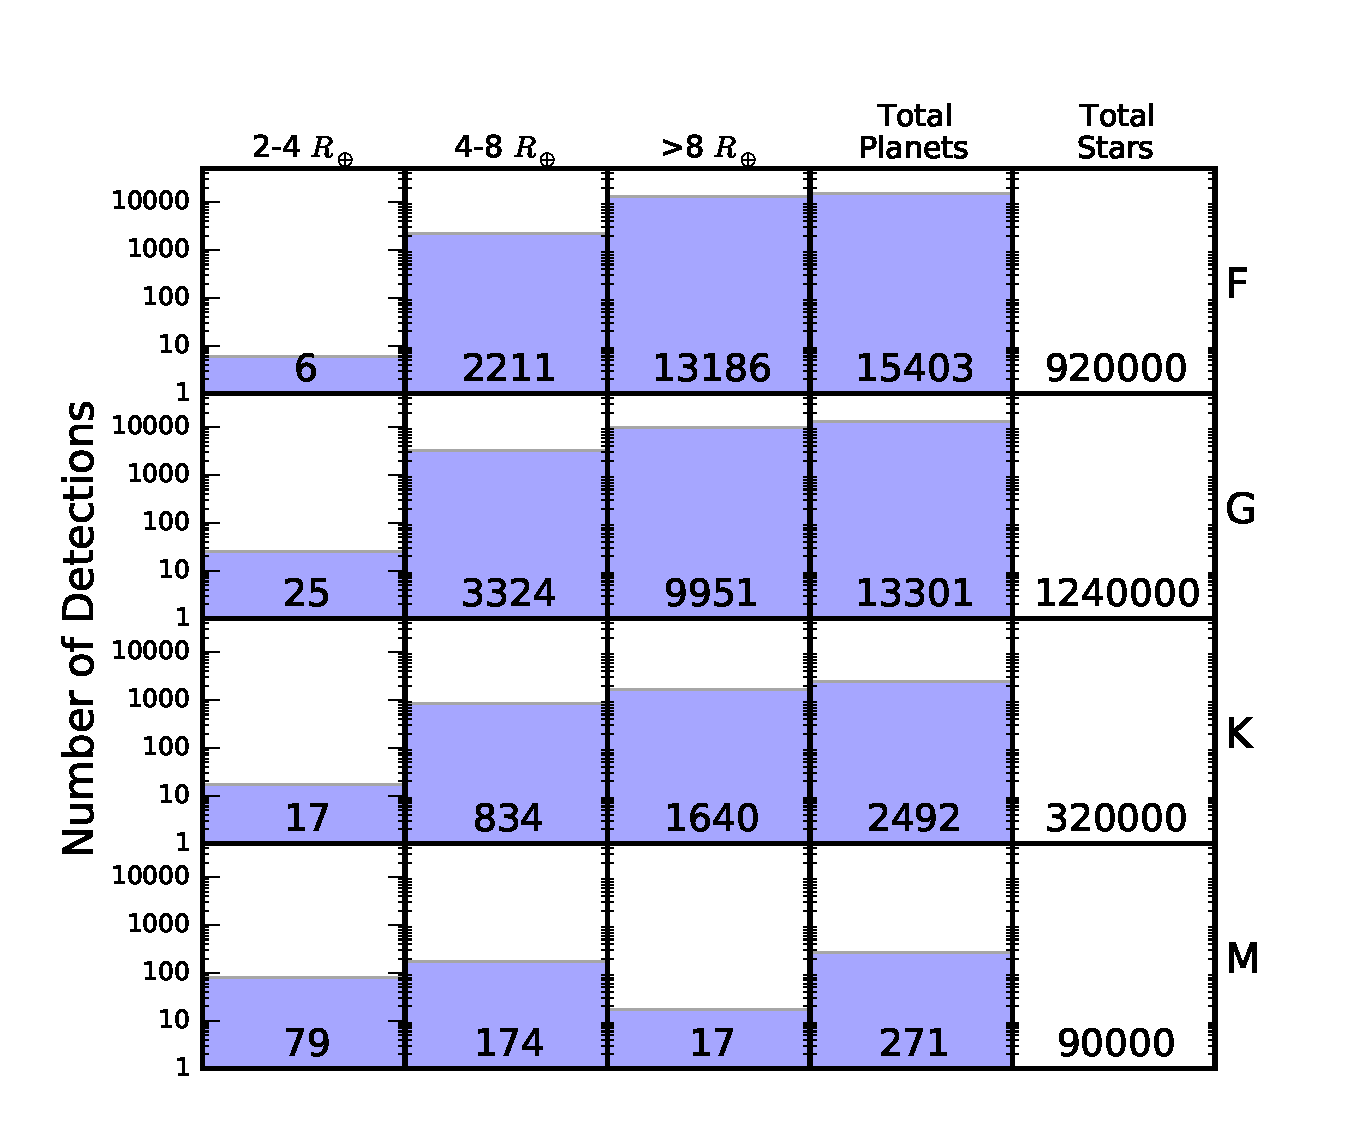
\includegraphics[width=0.75\textwidth]{chapter8/f5a_n.pdf}}
\caption[Expected transiting planet yield from \WF\ assuming giant planet occurrence follows the same
relation with metallicity as observed in the Solar neighborhood]{The same as Figure \ref{fig:yield1}, assuming planet occurrence for planets
larger than 5 \rearth\ follows
the relation with stellar metallicity as observed in the Solar neighborhood,
following \citet{JohnsonApps09}. Under these assumptions \WF\ will detect 
more than 30,000 planets.}
\label{fig:yield2}
\end{figure}



\section{Confirmation of Transiting Planetary Systems}
\label{sec:confirm}


The major challenge for transiting planet studies is to verify that the observed transiting object is a planet rather than a false positive. 
Multiple astrophysical events can be mistakenly identified as transiting planets. 
First, because of degeneracy pressure, Jupiters, brown dwarfs, and low-mass M stars all have similar radii \citep{Chabrier97}.
Hence, detection of a Jupiter-radius transit depth alone is insufficient to claim a planetary detection. 
Second, a false positive can occur in the case of blended light, when the star in 
question in the aperture is actually the combined light of multiple stars.
For example, a background unknown eclipsing binary could be blended with the primary target
star.
Similarly, the primary itself could be an eclipsing binary blended with the chance alignment
of a background star or the light of a hierarchical triple third star.
These degeneracies are easily resolved with RV observations, but those will not be possible for most \WF\ transit candidates.
However, previous studies have shown in the case of \kep\ that it is possible to validate transiting planet candidates by ruling out various false positive scenarios \citep{Morton12, Morton16}. Here and in Section \ref{sec:validate}, we explore various means to confirm, validate, or rule out false positives for \WF\ transiting planet candidates.




\subsection{TTVs}

The most straightforward way for \WF\ to confirm the planetary nature of transit signals from small
planets is through the detection of transit timing variations.
In Section \ref{sec:ttvs}, we showed that TTVs are easily recovered for a scaled-down version of the Kepler-9 system.
The exact nature of any TTV curve depends on the architecture of any particular TTV 
system: two planetary systems with identical planets but different orbital eccentricities,
arguments of periapse, or longitudes of ascending node would exhibit different TTV
signals. 

A full simulation of this stuff is beyond the scope of this paper. However, we note that
the TTV catalog of \citet{Holczer16} lists 571 \kep\ planet candidates with
TTV signals larger than 30 minutes and 176 with TTV signals larger than 60 minutes.
Many of these planets will be too small to be detectable in the relatively noisier
\WF\ data.
Considering these numbers,
based on the number of planets we expect \WF\ to be able to detect and the timing precision 
we expect the mission to achieve on individual transits \ref{sec:ttvs}, 
we expect more than 100 TTV detections over the observing campaign. 

\WF\ will have the added benefit of an observing baseline larger than five years, longer
than the original \kep\ mission. TTVs that manifest themselves on longer timescales, 
such as those caused by non-resonant planets, Roemer delay
from a hierarchical binary star, or orbital evolution of a giant planet in a short orbit \citep{Ragozzine09, Maciejewski16},
will be more likely to be detectable with \WF.

While TTVs will be extremely useful to confirm the planetary nature of small planets,
given the observing strategy of \WF\, it is unlikely that TTVs will be able to robustly
determine masses.
To verify this claim 
we use TTVFast \citep{Deck14} to integrate a dynamically interacting planetary system 
compare the result to the simulated transits from Section \ref{sec:ttvs}
during six hypothetical \WF\ observing seasons. 
We purposefully schedule the \WF\ seasons to coincide with the smallest observed TTV
signal to simulate a worst-case scenario.
For each observed transit, we add a random offset drawn from a uniform distribution on the
range [25 minutes, 40 minutes], similar to the predicted scatter on measurements of the times 
of individual transits, and assign an uncertainty on the observed time of transit
equal to this value. 

Fitting only the transits of the inner planet, we find that a dynamically interacting
planet model fit the data considerably better than a linear ephemeris ($\Delta \chi^2 = 72$). 
In this case, these planets would be easily confirmed via \WF\ observations:
only very contrived examples of planets with these masses, orbital periods, and 
eccentricities produce nondetectable TTVs. 
However, the inferred masses of the transiting planets are a function of the unknown
eccentricity: a pair of 10 \mearth\ planets or a pair of 25 \mearth\ planets can both
explain the observed TTVs.

In many cases, while confirmation of the planetary nature of systems will be easy, 
the large gaps between seasons will
complicate determination of unique solutions of the masses of individual planets
and induce
degeneracies between their masses and eccentricities.
For the brightest stars, it may be possible to identify particular transits that would
be useful for precise determination of planet masses and to follow up these planets with
ground-based
facilities at these specific times.


\subsection{Secondary Eclipses}


It is unlikely that TTVs will be useful for confirmation of more than a few of the 
hot Jupiters detected by \WF.
TTVs depend on the existence of a second planet, but
giant planets are most often detected in isolation, without a transiting companion
\citep{Steffen12c}.
There is only one hot Jupiter system with detected TTVs induced
by the presence of an additional planet \citep{Becker15}. 
However, it is possible that these planets will be confirmed by observations of their
secondary eclipses. The depth of the secondary eclipse yields a measurement of the
brightness temperature, and thus the flux in that bandpass \citep[e.g.][]{Charbonneau05}.

From \kep\ data alone it is difficult to confirm planets via secondary eclipses.
While \kep\ found thousands of planets, it was only able to confirm planetary systems
via detection of their phase curves and 
secondary eclipses for a handful of these \citep[e.g.][]{Esteves13, Quintana13, Angerhausen15}. 
Because the \kep\ bandpass spans approximately $0.4-0.9$ $\mu$m, near the peak of a typical
stellar spectrum but far bluer than the typical planetary spectrum, only the hottest,
largest planets are detectable by their own emission. 
However, \WF, with its primary bandpass spanning 0.927-2.000 $\mu$m, will be significantly 
more effective at observing planetary emission directly. 

To determine the feasibility of observing secondary eclipses with \WF, we consider the case of a hot Jupiter transiting a Sunlike star, similar to the
case of Section \ref{sec:HJ}. 
We can determine the relative flux of the two objects across the \WF\ bandpass to determine
the integrated secondary eclipse depth expected.
We assume a Jupiter-sized planet with an equilibrium temperature of 1200 K orbiting a 
Sunlike star.
We obtained a theoretical spectrum for a 1200 K and 5800 K object from the BT-Settl
spectral library of \citet{Baraffe15}, using the updated CIFIST2011\_2015 models.

We then integrate these spectra across the W149 filter, assuming a planet the size of 
Jupiter being eclipsed by a star the size of the Sun.
We predict, for this system, a secondary eclipse depth of 350 parts per million, approximately equal to the transit depth of a $2$ \rearth\ planet.
From Figure \ref{fig:Sensitivity}, we expect detections of secondary eclipses to be
rare around stars with $\textrm{W149} = 19.5$, but common around the million stars with 
W149 brighter than 15.0.
For the bright stars, we expect to detect approximately one-third
of planets of this size and orbital period in one season of \WF\ data, and nearly
all planets across the entire mission, so the same will be true for detecting secondary
eclipses. 

We are likely to recover secondary eclipses of the hottest planets even more effectively.
The planetary equilibrium temperature scales as $a^{-1/2}$, and hot planets are often 
inflated relative to their cooler cousins \citep{Charbonneau00, Showman02}, both increasing
the depth of the secondary eclipse:
WASP-12b's secondary eclipse depth across this bandpass is nearly 2 parts per thousand
\citep{Croll11, Stevenson14b}, corresponding to the same depth of a transit of a 
4.9 \rearth\ planet.
We can then expect observations of secondary eclipses to be useful for confirmation of
hot Jupiter systems.


Secondary eclipses will provide additional benefits to our understanding of the population
of transiting hot Jupiters beyond simply confirmation.
The timing of the secondary eclipse depends on the eccentricity vector $e \cos \omega$,
enabling statistical analyses of hot Jupiter eccentricities and detections of non-circular
planets, providing clues into the dynamics of hot Jupiter formation.


\section{Validation of Transiting Planetary Systems}
\label{sec:validate}


\subsection{Z087 Photometry}

Transits of a dark object across the face of a star should be, to first order, achromatic.
False positive events caused by eclipsing binaries, where multiple objects are
self-luminous, will have wavelength-dependent depth variations as different portions
of the stellar SEDs are sampled at different bandpasses.
Multiband photometry can then be used to separate transiting planets from 
background eclipsing binary events.

In the \WF\ mission, one data point will be collected every 12 hours in the Z087 filter,
or one data point for every 47 obtained in W149.
For the example of Section \ref{sec:HJ}, in which a hot Jupiter transits a Sunlike star with
a three-day period, only 24 data points will be obtained during the transit event in
Z087 over the entire mission, approximately one data point for every six transits.
The situation will be even worse for planets with longer orbital periods, or those 
at higher impact parameters and shorter transit durations.

We can assume that the transit ephemeris and orbital parameters are known from the W149 photometry used to detect planetary transit signals. Therefore, we only need
to fit three parameters
in the Z087 transit model: two to describe the limb darkening and one to describe the transit
depth.
For this case, fitting the Z087 photometry we measure a transit depth to a precision of 
3.7\%. Hence, an 11\% difference in transit depth between Z087 and W149 is the minimum detectable difference at $3\sigma$ confidence using data from the entire
mission. This is sufficient to rule out many, but not all, stellar false positives.

For example, a false positive M7 dwarf with a temperature of 2900 K and a radius equal to Jupiter's
has a flux density smaller than the Sun by a factor of 5.7 in the W149 filter and 11.6 in
the Z087 filter, leading to a 9\% change in the observed transit depth between the 
two filters.
An increase in the cadence of Z087 observations would be required in order to detect
these depth variations to identify false positives. 
Alternatively, as long as the orbit is aligned such that secondary eclipses are
observable from Earth, this star would induce a 2 ppt secondary eclipse, easily detectable with
\WF\ photometry. 
While Z087 photometry may be useful at the current cadence in extreme cases, secondary
eclipse photometry will be much more significant, as long as the companion's orbit is
aligned such that secondary eclipses are visible.

Validation could be complicated by the effects of starspots, both in the case where
the planet crosses starspots, affecting the light curve shape, and where starspots
are located at different latitudes, affecting the transit depth and out-of-transit flux. 
Due to the nature of the W149 bandpass, we expect spots to have a minimal effect
on the observed light curve. 
They will be more prevalent in the Z087 photometry, 
but still diminished relative to the \kep\ bandpass.


\subsection{Phase Curves}
\label{sec:PC}


Although a transit is the most obvious signal in a light curve of a planet orbiting a
star, the companion planet affects the observed light curve throughout its orbit.
Phase curve variations are the sum of three separate effects:
reflected light, relativistic 
Doppler beaming, and ellipsoidal variations. 
These variations have been discussed in previous work as a method to measure planetary
masses \citep{Faigler11, Mislis12}, to detect new transiting objects \citep{Faigler15b}, and to
understand the atmospheres of transiting planets \citep{Knutson07, Faigler15a}.
\citet{McDonald14} analyzed the ability of \textit{Euclid} to use phase curve
variations to confirm the planetary nature of transit signals.
Here, we consider similar ideas in the context of \WF.


\subsubsection{Doppler Beaming}

As a planet and host star orbit their mutual center of mass, changing the velocity of the
host star, the flux emitted from the star is beamed towards the direction of travel.
A consequence of special relativity, the signal is observable at the non-relativistic
speeds at which stars move during their orbits.
To first order, the amplitude of the beaming signal is 
\begin{equation}
\frac{F_D}{F_0} = (3-\alpha)\frac{K_s}{c}
\end{equation}
where $F_D$ is the amplitude of the signal, $F_0$ the flux from the stationary star,
$\alpha$ the shape of the SED at the observed wavelength, $K_s$ the
Doppler semiamplitude of the star, and $c$ the speed of light \citep{Loeb03}.
The SED is relevant because, as the star's velocity is modulated, the Doppler shift
affects what features of the stellar spectrum fall in our bandpass.
For most stars, the W149 filter will fall on the Rayleigh-Jeans tail of the SED,
where $\alpha = 2$.

For a typical hot Jupiter ($K \sim 150$ m s$^{-1}$), this amplitude will be
$\sim 0.5$ parts per million, well below the sensitivity of \WF. 
However, this effect will be useful for detecting more massive objects of similar radii
masquerading as 
hot Jupiters, such as brown dwarfs or very low mass stars.
A $50$ \mjup\ object with a three-day period would exhibit a 25-ppm signal.
From Section \ref{sec:small}, we determine we can measure a transit depth
to a precision of $40$ ppm. 
That transit event has a duration of 1.5 hours, while the beaming signal occurs
throughout the planet orbit, providing ample opportunity to detect a 25-ppm signal.


\subsubsection{Ellipsoidal Variations}

Ellipsoidal variations are an achromatic phenomenon caused by changes in the sky-projected
shape of a star as a planet orbits, affecting the star's gravitational potential.
The signal has twice the frequency of the planet's orbit. 
Following \citet{Loeb03}, to first order the magnitude of the signal is
\begin{equation}
\frac{F_E}{F_0} \sim \beta \frac{M_p}{M_s} \bigg(\frac{a}{R_s}\bigg)^{-3},
\end{equation}
Here, $\beta$ is a term which depends on the nature of gravity darkening for the host star.
For sunlike stars, this value is approximately 0.45. $M_p/M_s$ is the mass ratio between the planet and star and $a/R_s$ is the reduced orbital semimajor axis.

In general, the signal is of a similar magnitude to the Doppler beaming
signal, and only likely to be useful in separating brown dwarfs from planets:
transiting planets will only be notable by a nondetection of their ellipsoidal 
variations.

\citet{McDonald14} note that in the case of \textit{Euclid}, a color-dependence in observed
ellipsoidal variations would be a signature of a background eclipsing binary,
as the signal would be achromatic but the relative flux between the foreground 
and background target would vary between the two bandpasses. 
The same is true here, although with the cadence of Z087 observations we do not expect
this effect to be detectable.
In any cases where such an effect would be detectable, variations in the eclipse depth
between the bandpasses would also be detectable, likely at a much higher significance.




\subsubsection{Thermal Emission}


For planets with significant differences in their dayside and nightside 
surface temperatures, variations in the observed thermal emission from the planet will be
detectable.
The variation due to thermal emission depends on the difference in temperature between
the two sides of the planet, but for some systems can approach the entire depth of the
secondary eclipse \citep{Stevenson14a}, especially in the near-IR where \WF\ will observe.

The upcoming \textit{JWST} mission will provide detailed information about the 
thermal emission for particularly interesting, nearby systems. 
\WF, by comparison, will provide much less detailed information about any individual
system.
The data will be integrated over the entire W149 bandpass and at a considerably lower
precision than \textit{JWST}, but will be available for many more systems.

The ability to detect thermal emission in \WF\ data depends on the difference in temperature
between the day side and the night side of the planet.
Those planets that are tidally locked will thus be the most likely to exhibit a visible
signal in the phase curve. 
The same systems will be those for which secondary eclipses will be most readily visible.
Secondary eclipses only provide information about the dayside of the planet, while a 
phase curve will provide information at all longitudes.
Therefore, reflected light observations will likely be useful in concert with detections
of secondary eclipses to understand spatial variations in planetary atmospheres.

\subsection{Ground-based followup}

In principle, the transiting planet candidates discovered by \WF\ can be followed
up by adaptive optics (AO) systems on 30-meter class telescopes. 
These observations may not provide much leverage over the \WF\ data themselves.
The diffraction limit of a 30-meter telescope in $K$-band is $\sim 20$ milliarcseconds.
While considerably smaller than the \WF\ pixel scale of 0.11 arcsec pixel$^{-1}$, this still
corresponds to a projected separation of 20 AU for a star with W149 = 14.5 and 200 AU
for a star with W149 = 19.5, meaning many bound binary companions will be unresolved 
even when operating a thirty-meter telescope at the diffraction limit.


\section{Conclusions}


While ostensibly a microlensing mission, \WF\ will provide a 
tremendous opportunity for the study of short-period, transiting planets as well. We have shown in Section \ref{ss:yield} that if the occurrence rate of planets is the same as for the main \kep\ field, \WF\ will detect over 12,000 transiting planets with sizes as small as $2 R_{\oplus}$. If the occurrence rate scales with metallicity as in \citet{Johnson10a}, we expect a factor of $\sim 2.4$ more (i.e., ~30,000 planets) given that the \WF\ field is more metal rich than the Solar neighborhood.

To maximize the opportunity that \WF\ provides, we emphasize a few points to be considered 
during the 
design of the instrument.
Since more small planets detected by \WF\ will be confirmed via observations of 
TTVs than any other method, the long baselines during which these TTVs can manifest
themselves are essential. 
The current strategy, through which multiple fields are observed in parallel, cycling
every fifteen minutes, provides an ideal arrangement to observe TTVs.
For this strategy, it is imperative that the time between observations is small relative
to the typical transit duration so that individual transits can be well-timed.

Giant planets, meanwhile, will be most efficiently confirmed via analysis of their 
secondary eclipses. 
The near-IR bandpass will enable robust determination of the luminosity of the 
transiting companion, allowing for differentiation between planets and self-luminous 
low-mass stars. 
$Z$-band photometry could also provide useful data for this goal, both during the primary
transit and secondary eclipse. 
As currently imagined, the 12-hour cadence of $z$-band photometry does not provide enough
data in transit or eclipse to confirm systems as real or as definitive false positives.
An increased rate of $z$-band photometry, perhaps as often as once every three hours, 
would provide more opportunities to separate transiting hot Jupiters from self-luminous
brown dwarfs or giant planets.
If an increase in the rate of Z087 photometry at the expense of W149 photometry does not
have a significant effect on the expected yield from the primary microlensing mission, 
and if the time to change filters is small relative to the time to slew from one field to the 
next, we urge the \WF\ team
to consider an increased rate of Z087 photometry.



The majority of transiting planet detections will be around faint stars, as these stars
will make up the majority of observed stars in the sample.
We expect saturated dwarf stars (with W149 $< 15$) to account for fewer than 100 
planet detections. 
Photometry for these bright stars has been considered for the purposes of asteroseismology
\citep{Gould15}.
It will also be important for transiting planets: although these make up only a small
fraction of the total planet yield, the low levels of photon noise mean these stars 
produce the highest sensitivity to the smallest planets observable with \WF.
Additionally, these planets will be nearest transiting planets to Earth discovered by \WF\
as well as the ones most easily able to be followed up by other facilities on the ground
and in space for detailed characterization.
Thus, effort should be made to achieve precision photometry on these saturated stars.

In this work, we assume the noise from \WF\ will be purely white, with the correlated 
noise negligible compared to its uncorrelated counterpart.
Given the large levels of white noise expected (1 mmag for the brightest stars) this is
not an unreasonable expectation.
Observations of TTVs, a time-sensitive phenomenon, require a proper understanding of the
noise \citep{Pont06}.
We hope the \WF\ team will make every effort to understand the noise properties of the detector before launch.



